\chapter{IRRADIANCE MONITORING NETWORK}
\label{chap:sens_net}

This chapter describes the irradiance monitoring network that was
deployed in Tucson, AZ, and is the basis for much of the forecasting
work in this dissertation.
First, we present some background on why we built the network.
Next, we describe the design of the custom sensors that we deployed as
part of the network.
Then, we discuss how rooftop PV systems can be used as proxies for
irradiance sensors.
Finally, we present possible improvements one might consider for
future networks.

\section{Background}

The initial application of an irradiance monitoring network is laid
out in \cite{Lonij2013}.
Using historical data from 80 residential rooftop PV systems, Lonij
\etal produced intra-hour solar power forecasts that showed skill over
persistence forecasts.
The local electric utility (Tucson Electric Power) was interested in
receiving these short-term forecasts in real-time.
To generate real-time forecasts, data from sensors need to be gathered
in real-time, thus we set out building the irradiance monitoring
network that would report values in near real-time.

\section{Design of Custom Sensors}

why chosen?


\subsection{Photodiode Sensor}
\label{sec:photodiode}

teflon diffuser
scaled PD vs GHI, cosine rsponse

\subsection{Sensor Circuit}

A custom printed circuit board was designed for the components that
store and send sensor data to a central server every minute.
The circuit diagram for this board is shown in \Cref{fig:circuit}.
Design files for the circuit board can be found online \cite{sensorrepo}.

\begin{sidewaysfigure}[p]
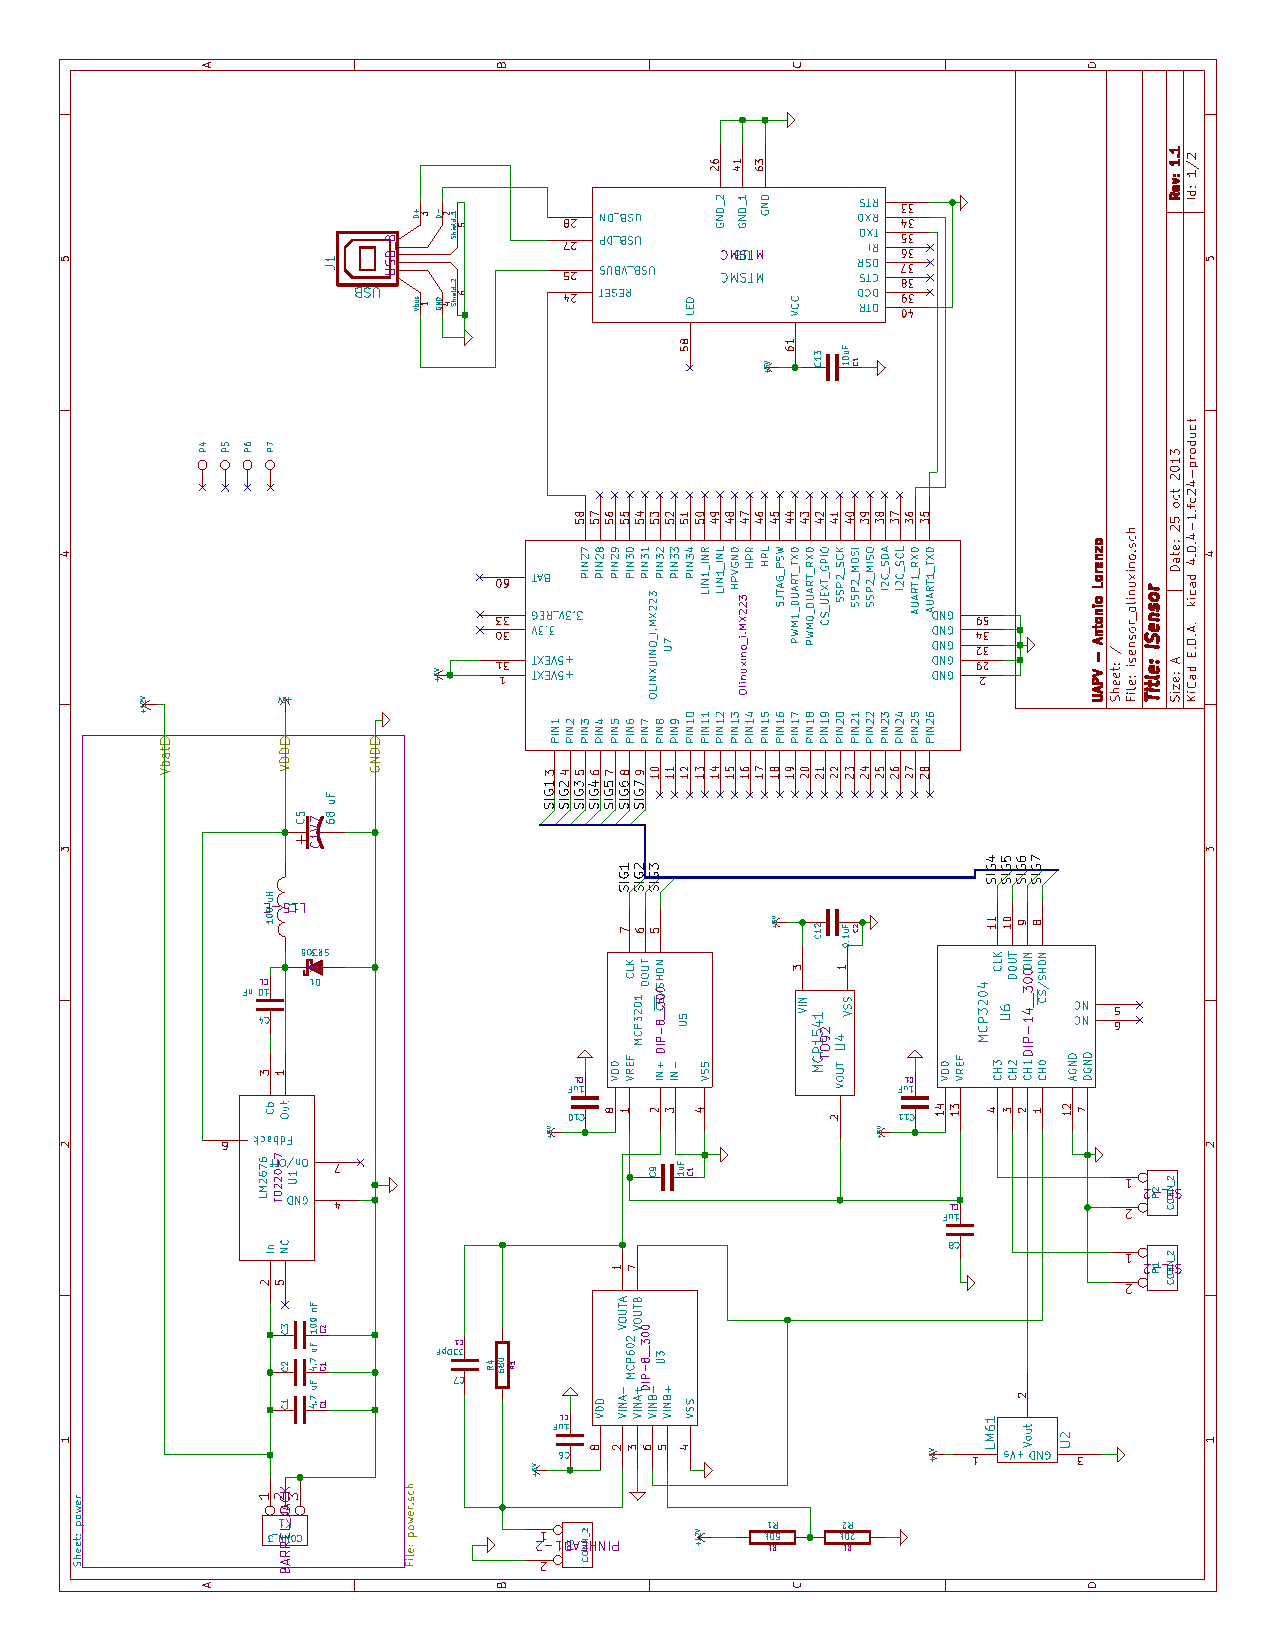
\includegraphics[angle=-90,width=\textwidth]{figs/circuit.pdf}
\caption[Custom sensor circuit diagram]{Circuit diagram for the
  custom, remote irradiance sensors.}
\label{fig:circuit}
\end{sidewaysfigure}

The custom sensors are developed around the Olimex
iMX223-OLinuXino-MICRO board.
The OLinuXino was chosen because it consumes little power ($< 1$W) and it
runs a full Linux operating system which allows for development in any
language that can be installed on Linux along with the usual suite of
Linux tools (SSH, Bash, logs).
It is also relatively inexpensive to purchase complete boards, and the
plans are open-source if one desires to build the board themselves.

Data is communicated via GSM using a MULTITECH MTSMC-H5-U SocketModem.
This modem accepts a standard SIM card that is registered with a
cellular data provider.
The modem is connected to the OLinuXino via USB.
WvDial and PPPD are used to setup the connection to the modem and
allow internet access.

Power to the system is provided by a 10W solar panel and a 6Ah
lead-acid battery.
A standard solar charge controller is used limit the current from the
panel to the battery.
The nominal 12V from the battery is routed to the circuit board with
the OLinuXino and modem and converted to 5VDC with a circuit based on
the LM2676 step-down regulator.

The sensor is designed to accept input from either a calibrated
pyranometer (Apogee SP-212) or an inexpensive silicon photodiode
(Osram BPW34) as discussed in \Cref{sec:photodiode}.
A trans-impedance amplifier (MCP602) with appropriate gain is used to
convert the current from the photodiode into a measurable voltage.

The voltage from the sensor (or sensor + trans-impedance amplifier) is
converted to a digital signal with the MCP3201 12-bit
analog-to-digital converter (ADC).
This digital signal is then read the OLinuXino at regular intervals
from the GPIO pins.
An additional 4 channel 12-bit ADC (MCP3204) is used to convert other
values such as enclosure temperature (measured by an LM61) and battery
voltage to be read on the OLinuXino GPIO pins for monitoring.
A 4.096V voltage reference (MCP1541) is used by both ADCs.

\subsection{Sensor Software}

reverse SSH

\subsection{Possible Improvements}

enclosure

new low power comps

integrated charge controller

lithium battery

gps location + time


\section{Rooftop PV Systems as Sensors}

One major challenge with using rooftop PV systems as sensors is that
the data is often difficult to collect.
One solution we employed is to use the built-in capabilities of some
inverters to send data directly via FTP.
With the help of a local PV system installer, Technicians for
Sustainability, we are collecting 5 minute averaged power data from
over 70 systems in the Tucson area in near real-time.
Since many inverters connect to a home owners network, we also
explored using cheap Linux devices (Raspberry Pi) to communicate with
inverters on the network and upload the data to a central server.

The electric utilities also have access to inverter data, although it
may be delayed by days or weeks and aggregated to daily or longer values.
With an increase in the installation of smart inverters, utilities are
increasingly able to access inverter data in real-time.
With an appropriate data transfer system in place, one can acquire
the rooftop data from the utility, generate a forecast, and send the
forecast back to the utility.

Since irradiance is the primary driver of PV output power, power data
from rooftop PV systems can act as a proxy for irradiance.
When analyzing both power and irradiance data, a units conversion is
likely necessary.
In our work, we choose to convert all irradiance proxy data to
clear-sky index
\begin{equation}
\label{eq:clrind}
k_n(t) = \frac{y_n(t)}{y_n^{clr}(t)}
\end{equation}
where $y_n(t)$ is the measured time-series and $y_n^{clr}(t)$ the
expected time-series for sensor $n$ if the sky were clear.
This approach accounts for differences in systems such as orientation,
peak power, and shading.
Furthermore, it detrends the diurnal cycle in the data.
The clear-sky expectation should account for temperature and aerosol
effects on a given sensor in some way to produce an unbiased clear-sky
index.

\section{Network Deployment}


%%% Local Variables:
%%% mode: latex
%%% TeX-master: "dissertation"
%%% End:
